\documentclass{article}
\usepackage{amsmath,amssymb,amstext,mathtools,array,url,bm,graphicx,color,epsfig}
\usepackage{fullpage,setspace}
\usepackage{authblk}
\usepackage{filecontents}
\usepackage{natbib}
\usepackage{lineno}
\usepackage[colorlinks]{hyperref}
\usepackage{subcaption}
\usepackage{float}
\usepackage[flushleft]{threeparttable}

\def\dt{\partial t}
\def\dx{\partial x}
\def\dy{\partial y}

\def\dz{\partial z}
\def\BE{\begin{equation}}
\def\EE{\end{equation}}
\def\half{\frac{1}{2}}
\def\calT{\cal T}
\def\Deltax{\Delta x}
\def\Deltat{\Delta t}
\DeclareSymbolFont{largesymbolsA}{U}{txexa}{m}{n}
\DeclareMathSymbol{\varprod}{\mathop}{largesymbolsA}{16}

\newtheorem{theorem}{Theorem}
\newtheorem{acknowledgement}[theorem]{Acknowledgement}
\newtheorem{algorithm}[theorem]{Algorithm}
\newtheorem{axiom}[theorem]{Axiom}
\newtheorem{case}[theorem]{Case}
\newtheorem{claim}[theorem]{Claim}
\newtheorem{conclusion}[theorem]{Conclusion}
\newtheorem{condition}[theorem]{Condition}
\newtheorem{conjecture}[theorem]{Conjecture}
\newtheorem{corollary}[theorem]{Corollary}
\newtheorem{criterion}[theorem]{Criterion}
\newtheorem{definition}[theorem]{Definition}
\newtheorem{example}[theorem]{Example}
\newtheorem{exercise}[theorem]{Exercise}
\newtheorem{lemma}[theorem]{Lemma}
\newtheorem{notation}[theorem]{Notation}
\newtheorem{problem}[theorem]{Problem}
\newtheorem{proposition}[theorem]{Proposition}
\newtheorem{remark}[theorem]{Remark}
\newtheorem{solution}[theorem]{Solution}
\newtheorem{summary}[theorem]{Summary}
\newenvironment{proof}[1][Proof]{\noindent\textbf{#1.} }{\ $\square$}


\begin{document}
\title{\bf Supporting Information: Comparative anatomy of geophysical flow models and modeling assumptions using uncertainty quantification}
\author[1,3]{Abani K. Patra}
\author[2]{Andrea Bevilacqua}
\author[1]{Ali Akhavan-Safaei}
\author[4]{E. Bruce Pitman}
\author[2]{Marcus I. Bursik}
\author[2]{David Hyman}

\affil[1]{\textit{Dept. of Mech. and  Aero. Eng., University at Buffalo, Buffalo NY 14260} }
\affil[2]{\textit{Dept. of Geology, University at Buffalo, Buffalo NY 14260} }
\affil[3]{\textit{Comp. Data Science and Eng., University at Buffalo, Buffalo NY 14260} }
\affil[4]{\textit{Dept. of Materials Design and Innovation, University at Buffalo, NY, 14260}}

\date{\texttt{\{abani,abevilac,aliakhav,pitman,mib,davidhym\}@buffalo.edu}}

\maketitle
\tableofcontents
\newpage
Supporting Information includes the local plots of Froude Number, the spatial integrals of force terms, and the local force terms contributions.

\section{Results of small scale flows on inclined plane and flat runway}
\subsection{Froude Number}
Figure \ref{fig:Ramp-Fr} shows the Froude Number, $\Vert \underline{\mathbf{u}} \Vert/\sqrt{gh}$, at the points $(L_i)_{i=1,\dots,4}$, for the three rheology models.
\begin{figure}[H]
         \centering
        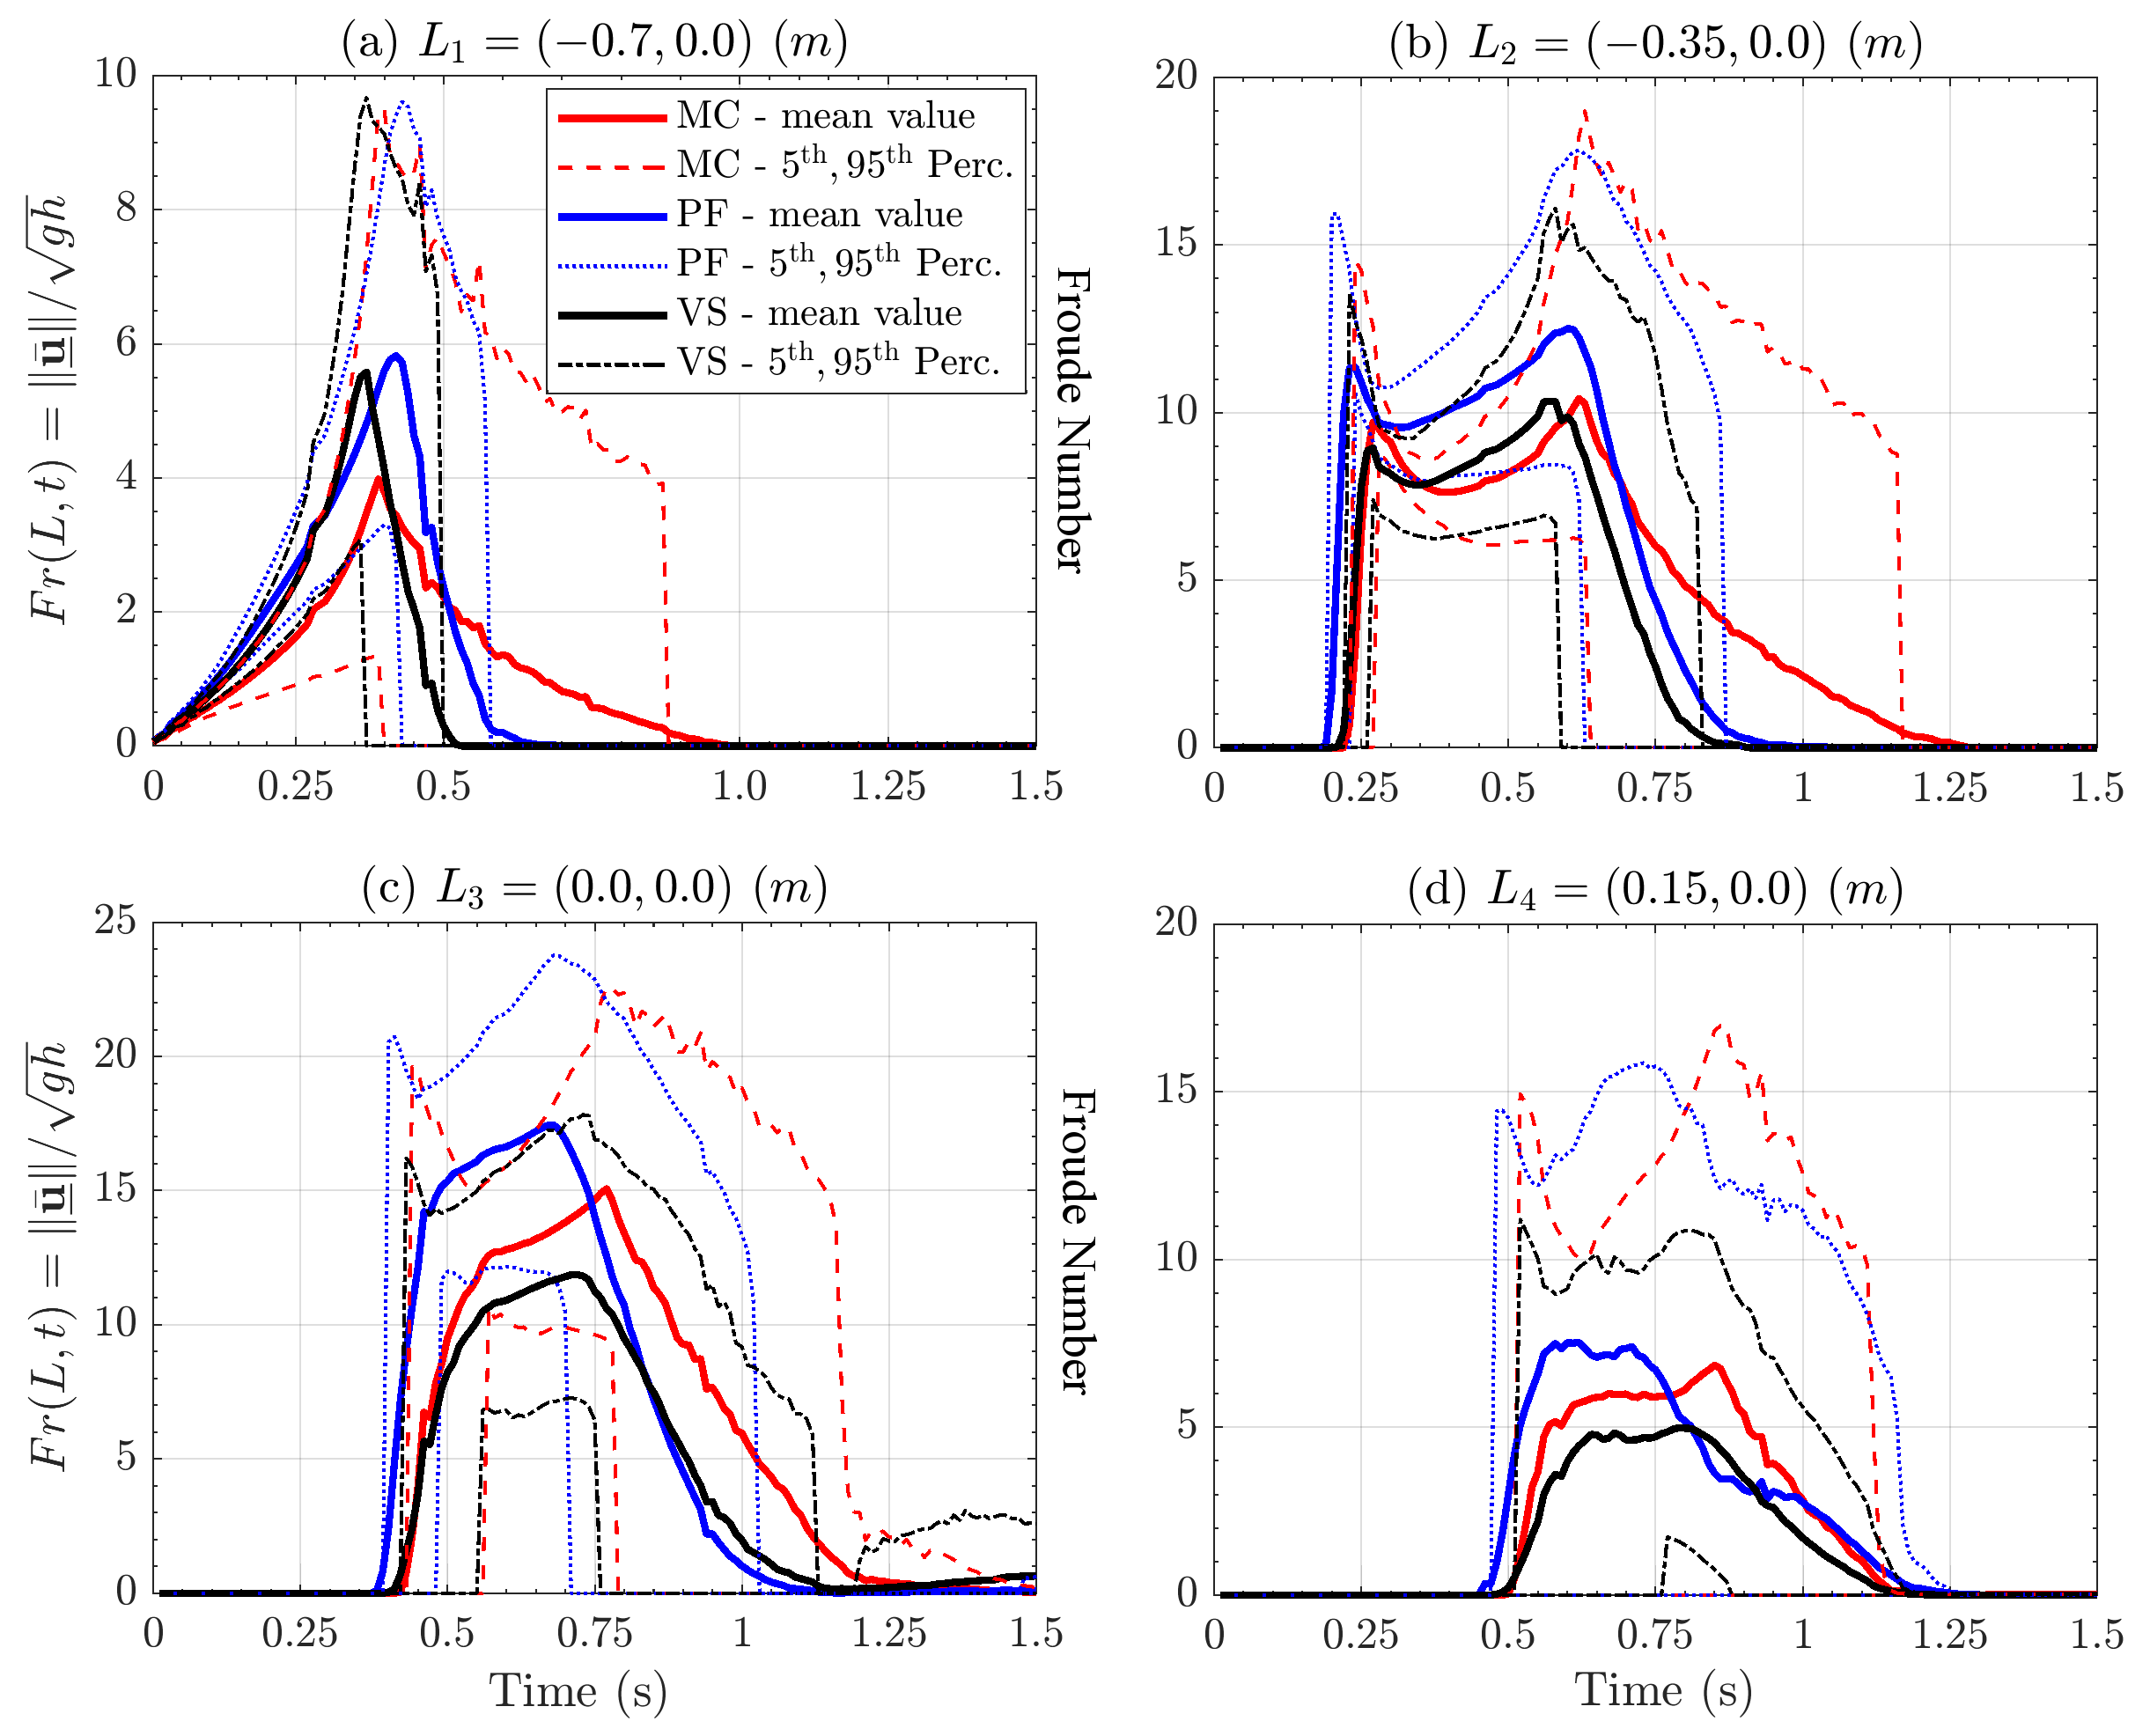
\includegraphics[width=1\textwidth]{InclinedPlane/LocalMeasurments/Froude.png}
        \caption{Records of Froude number at four spatial locations of interest. Bold line is mean value, dashed/dotted lines are 5$^{\mathrm{th}}$ and 95$^{\mathrm{th}}$ percentile bounds. Different rheology models are displayed with different colors. Plots are at different scale.}
        \label{fig:Ramp-Fr}
\end{figure}
Froude Number combines the estimates of flow height and speed. In plot \ref{fig:Ramp-Fr}a, related to point $L_1$, $Fr$ maximum average value is smaller for the MC model, $\sim 4$, than for the others, $\sim 6$. However, UQ tells us that 95$^{\mathrm{th}}$ percentile almost reaches $\sim 10$ in all the three models. After the peak, the values decrease slower and more concavely in MC model than in the others. In plot \ref{fig:Ramp-Fr}b, related to point $L_2$, $Fr$ shows a bimodal profile in time, with two separate peaks at $\sim 10$ on average, but reaching $\sim 18$ in the 95$^{\mathrm{th}}$ percentile plot. In fact, first maximum, at $\sim 0.25$ s is due to the speed peak, and second, at $\sim 0.6$ s is related to $\sqrt{h}$ decreasing while the speed is not significantly changing. In plot \ref{fig:Ramp-Fr}c and \ref{fig:Ramp-Fr}d, related to points $L_3$ and $L_4$, bimodality is less accentuated and becomes a plateau profile in $\sim [0.5, 0.75]$ s. PF model gives significantly larger $Fr$ values, even $>20$ at $L_3$, due to a larger speed and a thinner flow. It is worth noting, for the sake of PF model, that $Fr>\beta$ and the flow is in the dynamic regime during the most of the time.

\subsection{Force terms}
Figure \ref{fig:Ramp-Fx-spatial} shows the spatial integral of the force terms in the slope direction, for the three rheology models. The spatial integration is performed on half spatial domain, due to the symmetry with respect to the flow central axis. In plot \ref{fig:Ramp-Fx-spatial}a $\boldsymbol{RHS_1}$ represents the effect of the gravity in all the models. It starts with a plateau at $\sim 1.3 N$ before $\sim 0.55 s$, then decreases to zero after the material crosses the change in slope. The force values are consistent with the expression $\rho \left(V/2\right) g_x$, representing half the weight of material, projected along the slope direction. Uncertainty range of $\pm 0.2 N$ on the peak values. MC decreases slower, and has a more significant uncertainty, after the change in slope. PF decreases faster. In plot \ref{fig:Ramp-Fx-spatial}b $\boldsymbol{RHS_2}$ represent the friction at the base of the flow. It is negative and opposed to the gravity. A similar profile is shared by the three models, with a first short-lasting weakening before $\sim 0.1 s$, a plateau with a small strengthening after $\sim 0.5 s$, and a final waning after $\sim 1 s$, at the conclusion of the dynamics. MC does not reach zero, while the other models do. VS values are generally $\sim 0.5 N$ weaker than MC, and PF is intermediate, except in the initial peak, where it is the weakest. Strongest forces are reached during the plateau, and are $\sim -0.55 N$, $\sim -0.75 N$, $\sim -0.9 N$, with uncertainty range of $\pm 0.25 N$ in the plateau. Uncertainty is reduced in the final stages of VS and PF, but increases in MC. In plot \ref{fig:Ramp-Fx-spatial}c $\boldsymbol{RHS_3}$ is related to the curvature effects, and is not null only at the change in slope. It is always negative, i.e. reducing flow velocity, indeed it is equivalent to the friction due to the additional weigh generated by centrifugal forces. Its scale is ten times smaller than the previous plots, with values above $0.1 N$ only in MC. VS displays a bimodal profile, with a second and weaker peak at $\sim 0.75 s$. In plot \ref{fig:Ramp-Fx-spatial}d $\boldsymbol{RHS_4}$ is related to the additional forces of the models, differently characterized. In MC and PF, they are significantly small forces before $0.1 s$, completely negligible later. In VS, this is the velocity dependent term. It is negative and plays a significant role. It reaches $\sim 1 N$ at the change in slope, with uncertainty $\pm 0.3 N$. It is bell shaped and null before $\sim 0.1 s$ and after $\sim 1 s$. In plot \ref{fig:Ramp-Fx-spatial}e $\sum^4_{i=1}\boldsymbol{RHS_i}$ represents the total force in the slope direction, and summarizes the previous plots. The profile is characterized by a positively valued stage at $\sim 0.5 N$ before the change in slope, and by a negatively valued stage after that, with bell-shaped profile, and a peak at $\sim -0.5 N$. In the first stage MC is more flat, while PF and VS decrease. In the second stage MC is occurring later in time, of $\sim 0.1 s$; PF and VS are remarkably similar, but VS wanes faster.
\begin{figure}[H]
        \centering
        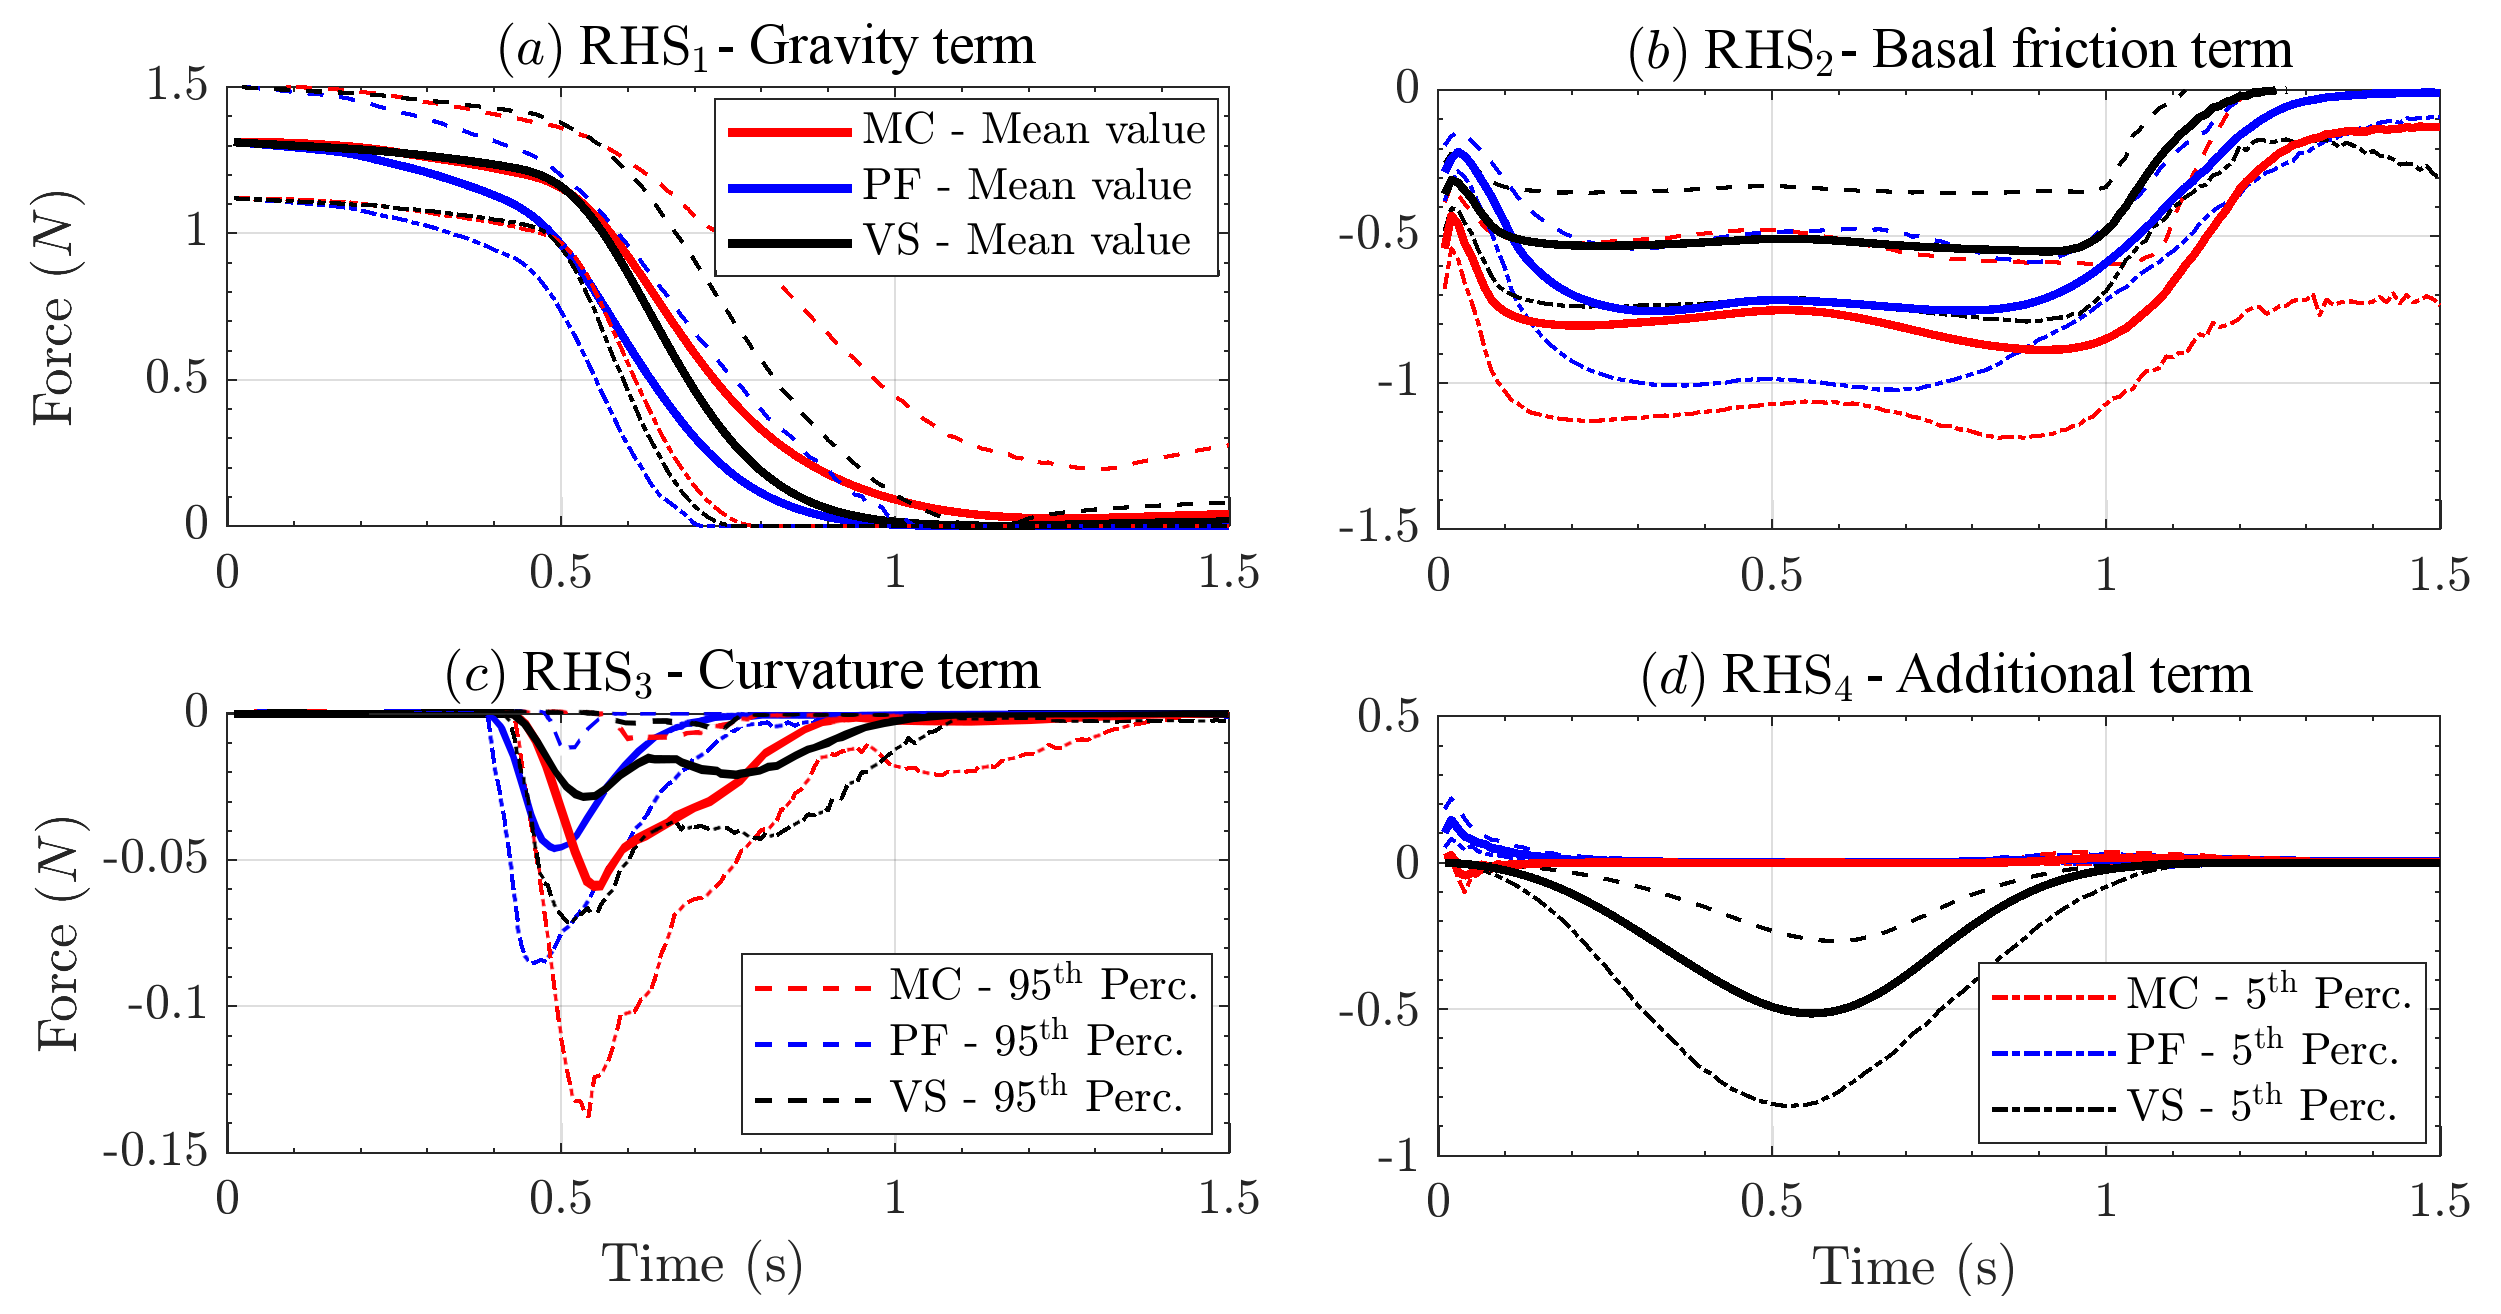
\includegraphics[width=1\textwidth]{InclinedPlane/AveragedMeasurments/ForcesIncline.png}
        \caption{Spatial sum of the RHS forces in the slope direction. Bold line is mean value, dashed lines are 5$^{\mathrm{th}}$ and 95$^{\mathrm{th}}$ percentile bounds. Scale of plot (c) is ten times larger than in (a),(b),(d); scale of plot (e) is slightly smaller.}
        \label{fig:Ramp-Fx-spatial}
\end{figure}
\newpage
\section{Results of large scale flows on the SW slope of Volc{\'a}n de Colima (MX)}
\subsection{Froude Number}
Figure \ref{fig:BAF-Fr-MC} shows an overview of the mean Froude Number, $\Vert \underline{\mathbf{u}} \Vert/\sqrt{gh}$, at the 51 spatial locations of interest, according to MC.
\begin{figure}[H]
         \centering
        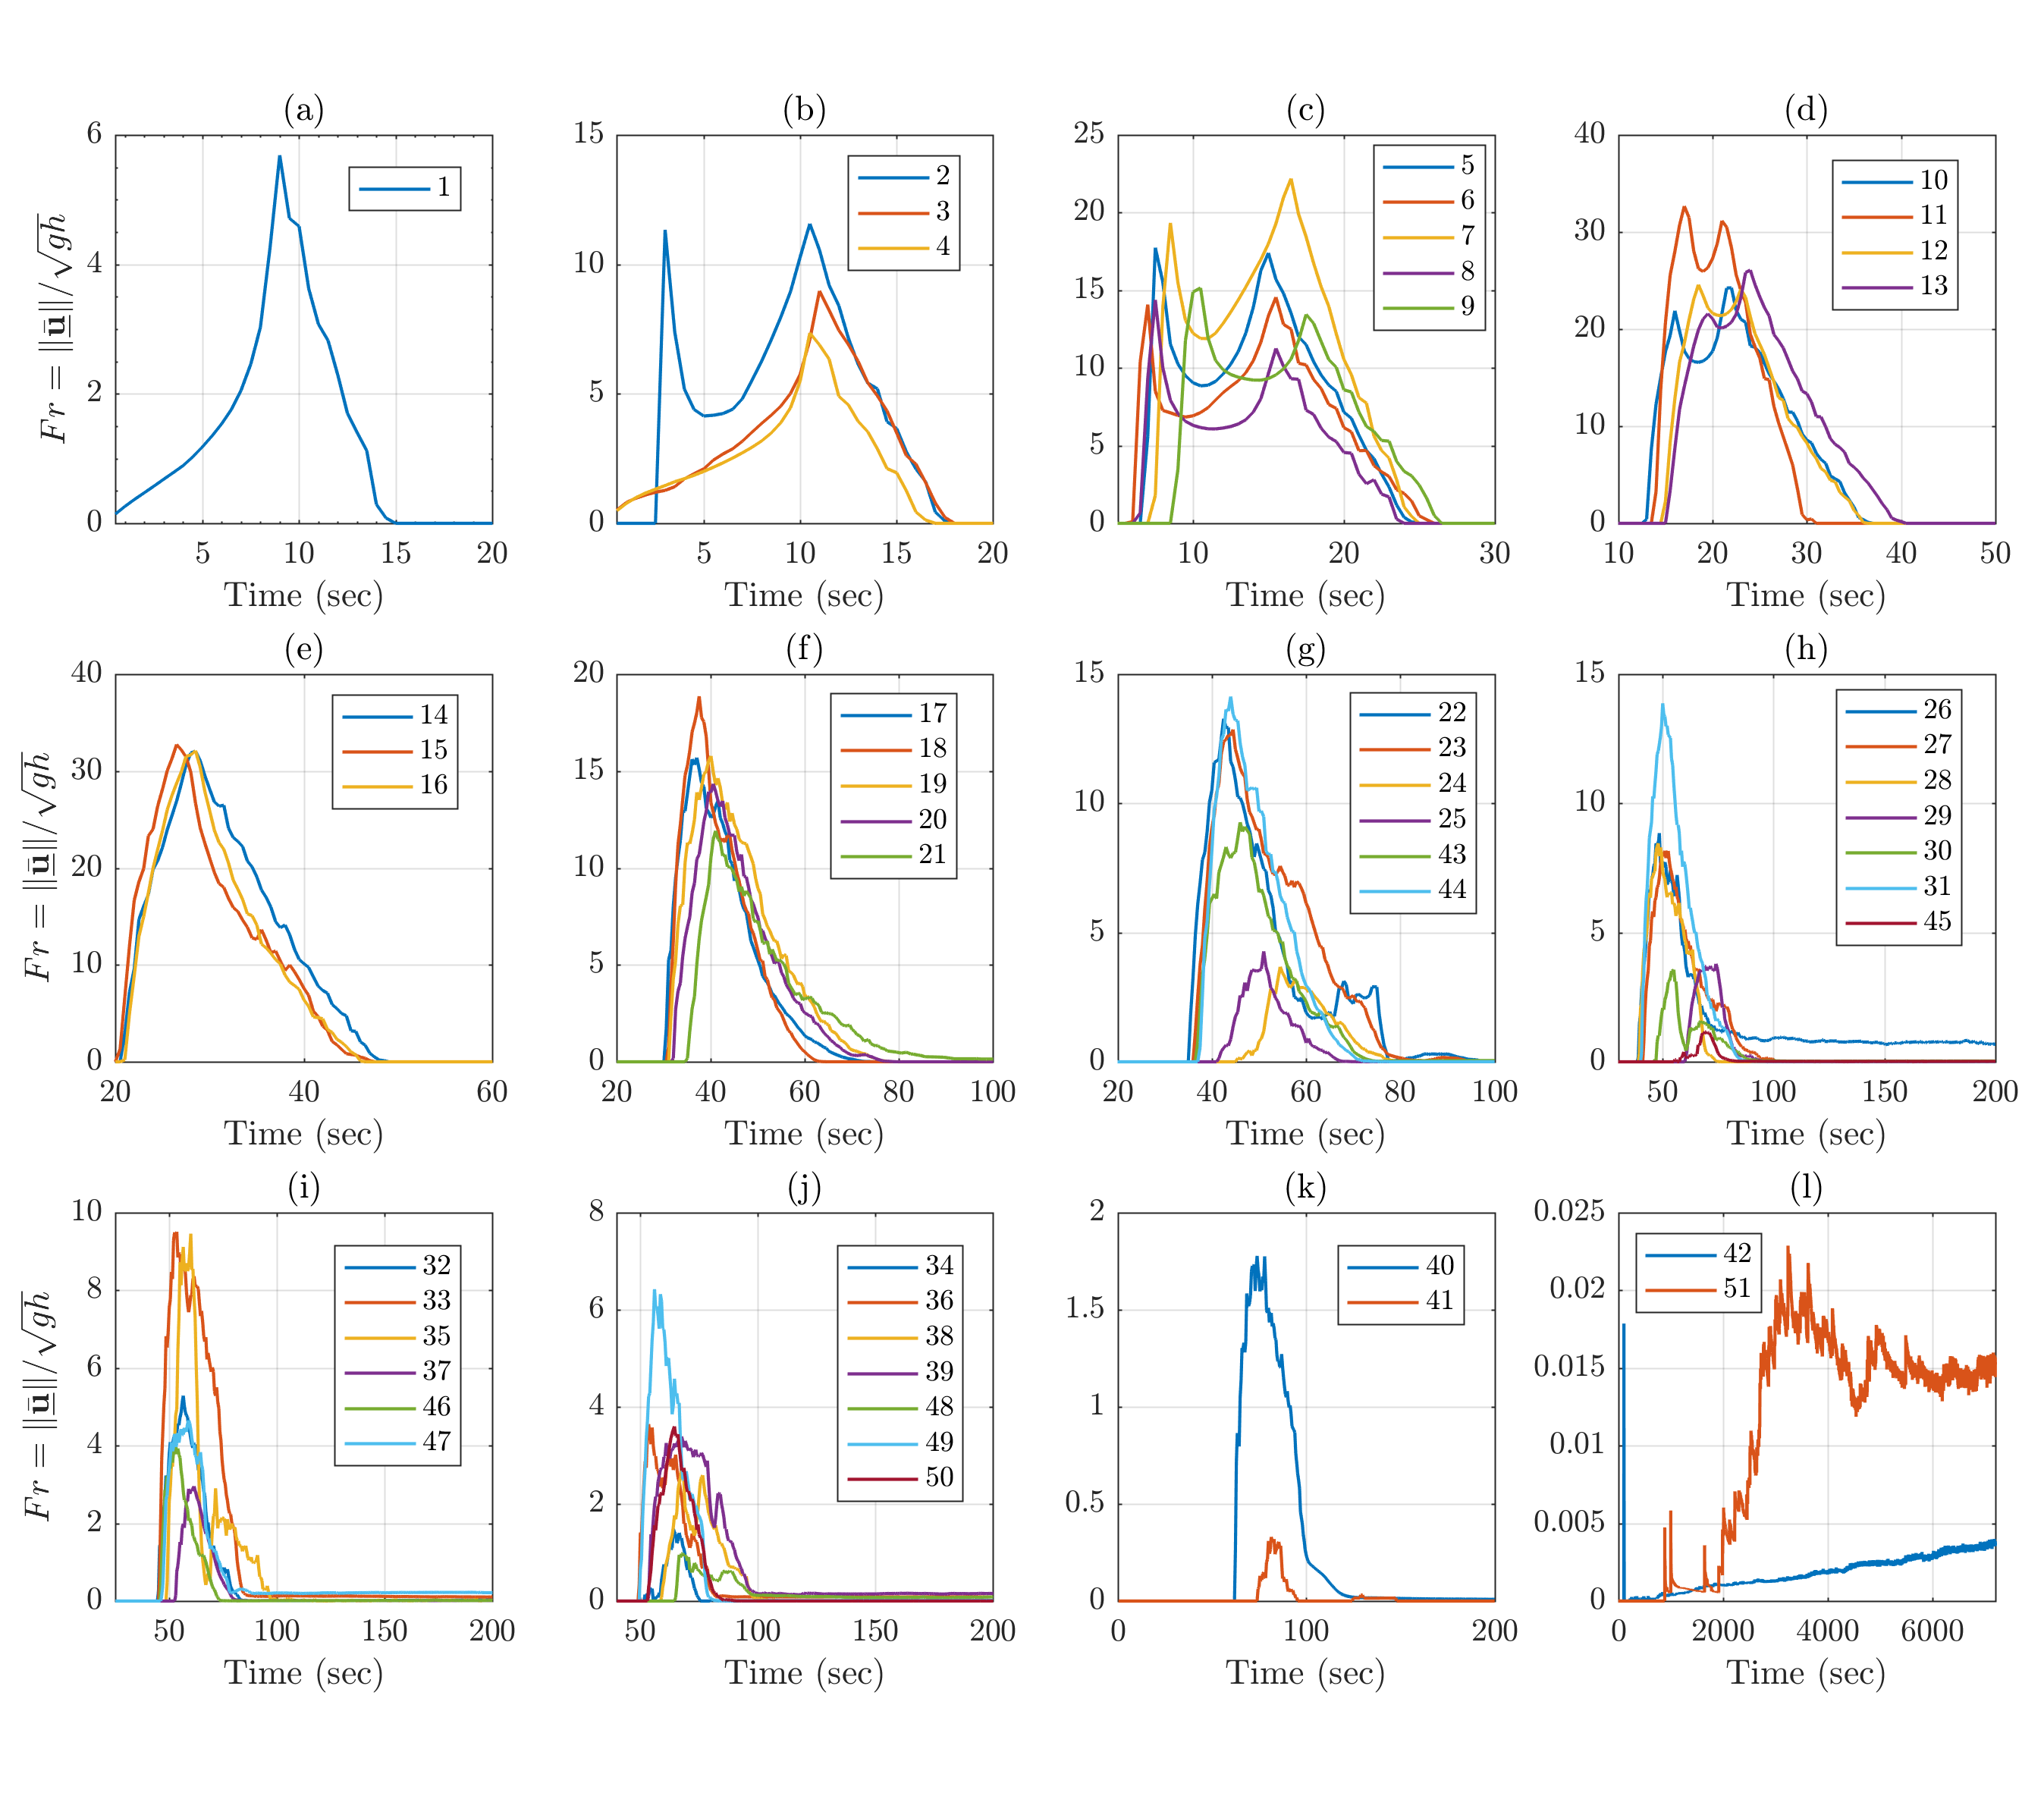
\includegraphics[width=1\textwidth]{MC&VS_51/Froude_MC2.png}
        \caption{MC model, records of average Froude Number in 51 spatial locations of interest.}
        \label{fig:BAF-Fr-MC}
\end{figure}
Froude Number combines height and speed measurements, and plot profiles are similar to what observed in Figure \ref{fig:Ramp-Fr}. In particular, in plots \ref{fig:BAF-Fr-MC}b,c,d, strongly bimodal profile are observed due to the interplay between flow height and flow speed. In plots \ref{fig:BAF-Fr-MC}f,g,h,i,j, sharp changes are observed, and the plots are significantly rough when the speed is significantly small.

Figure \ref{fig:Colima-Fr1} displays Froude Number, $\Vert \underline{\mathbf{u}} \Vert/\sqrt{gh}$, at the selected locations $(L_i)_{i=8,10,17,39,43,46}$, for the three rheology models.
\begin{figure}[H]
         \centering
        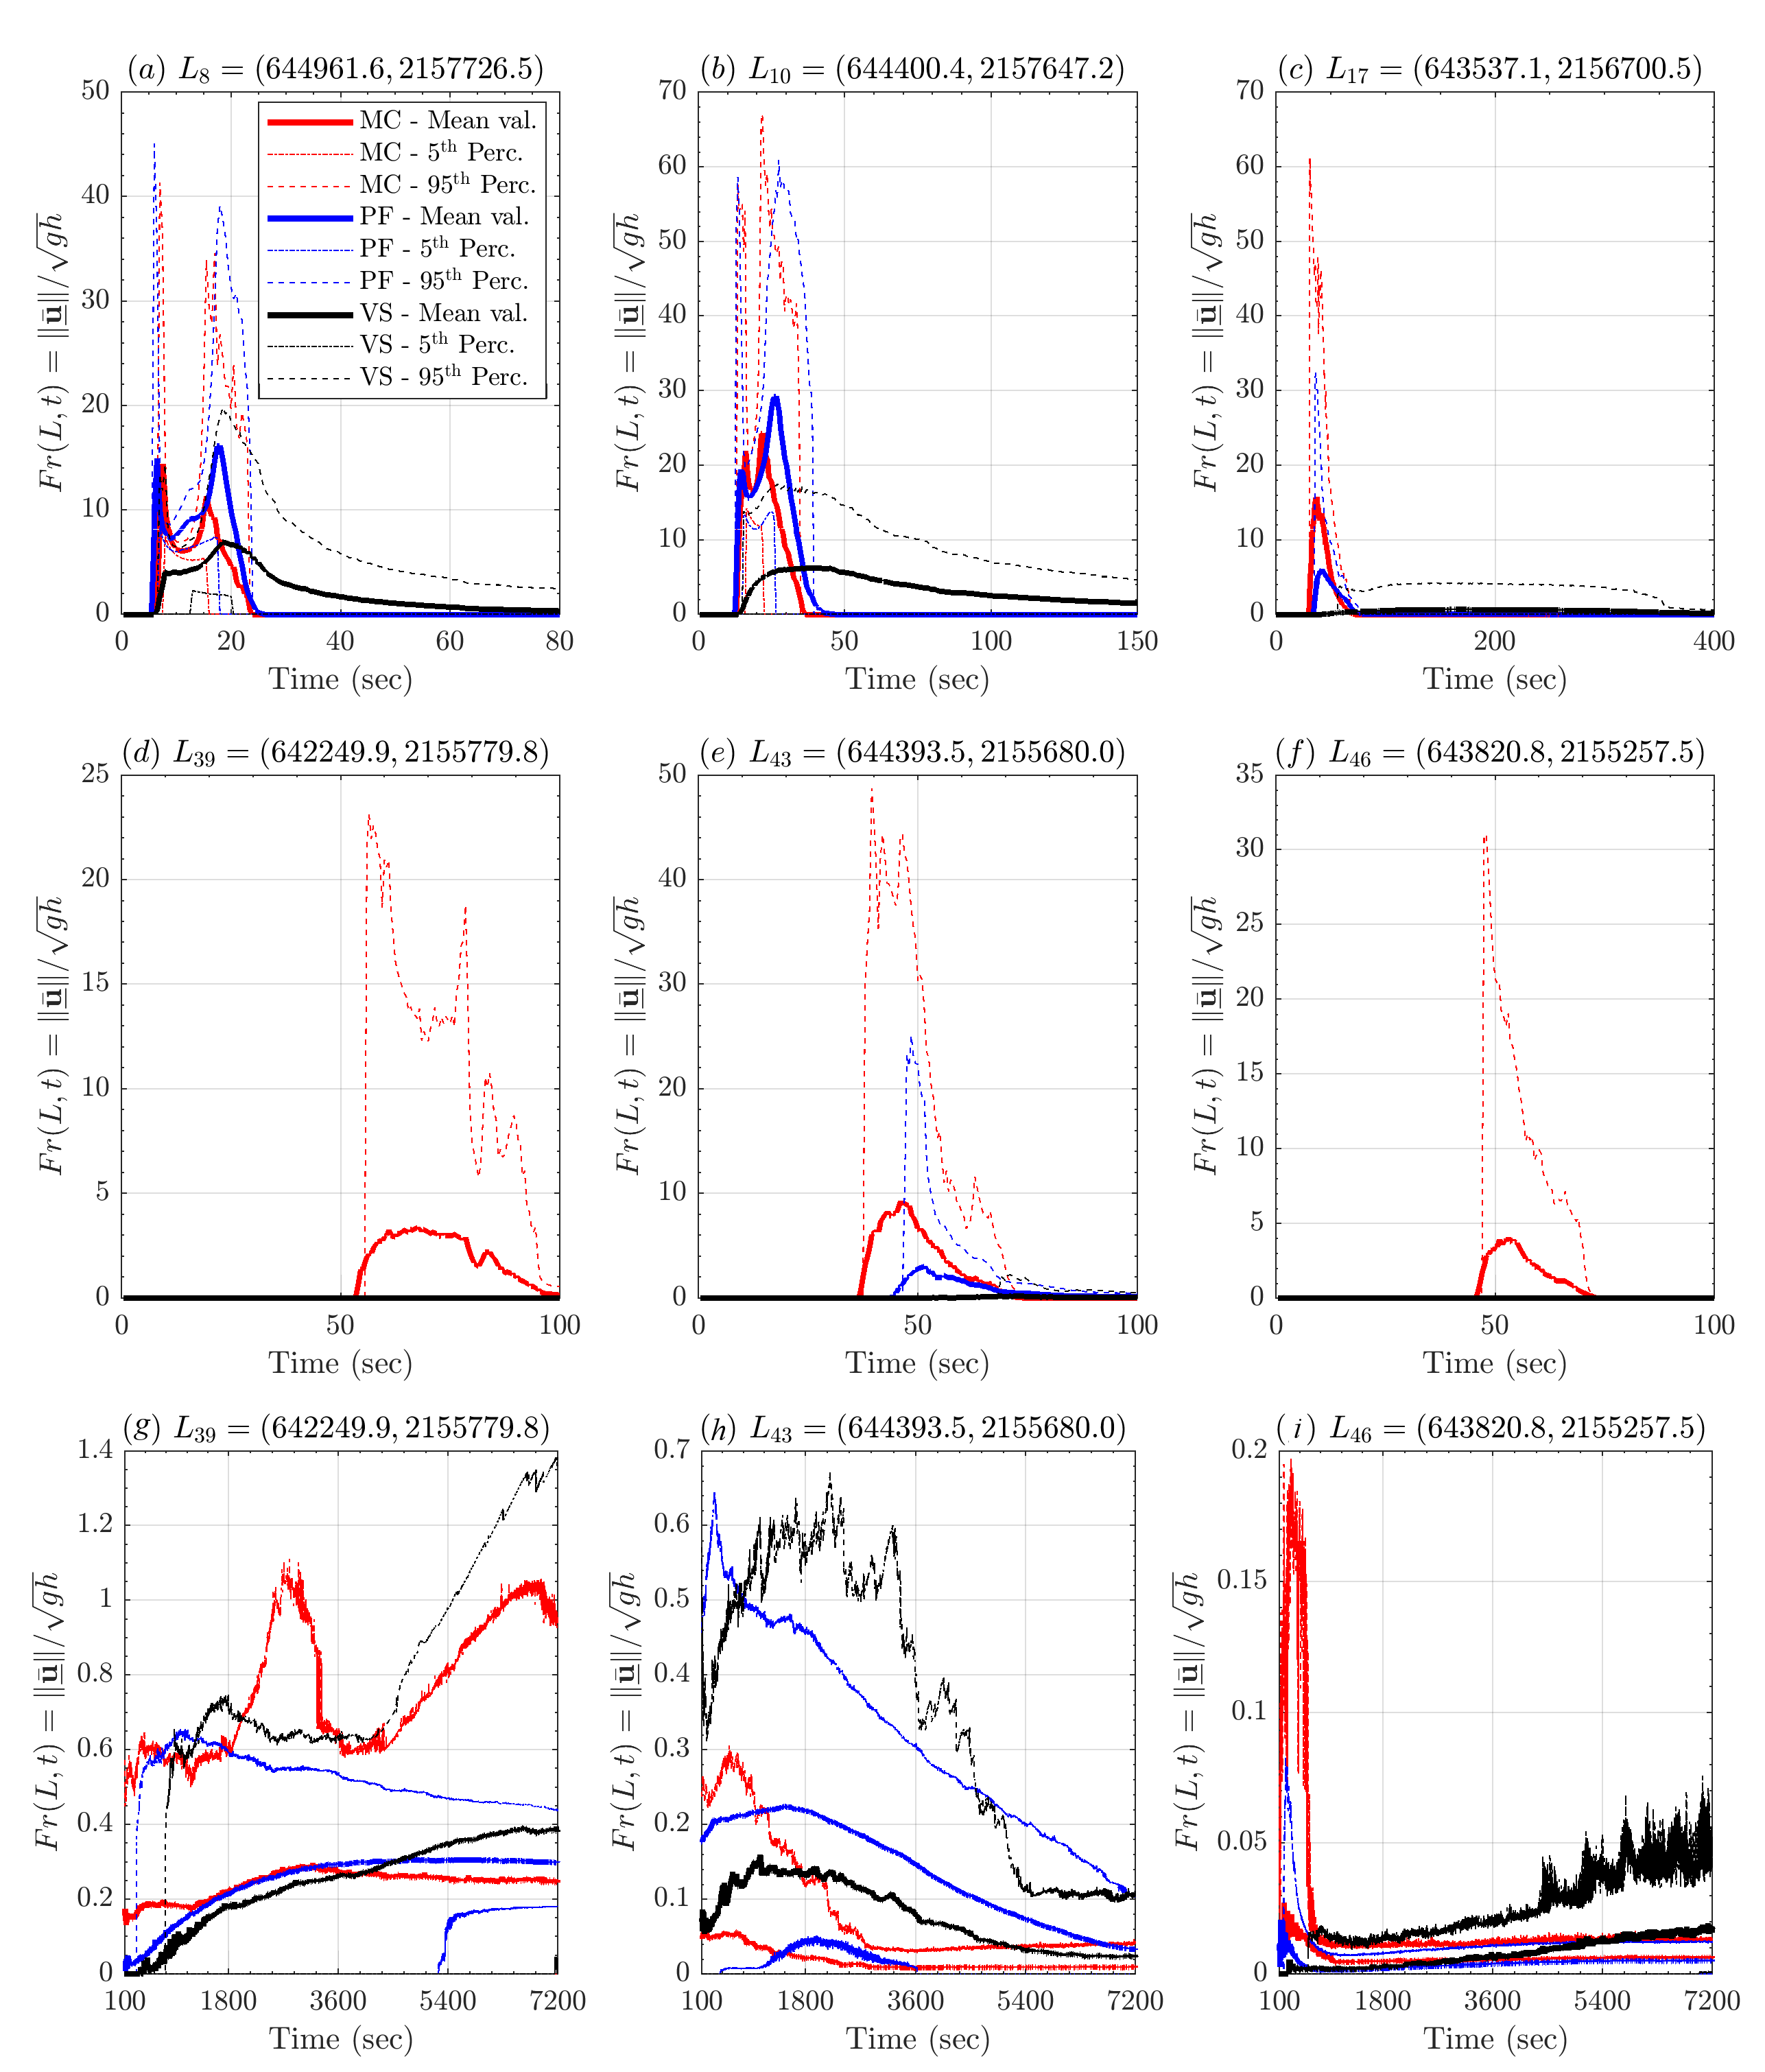
\includegraphics[width=1\textwidth]{BAF_VolcanDeColima/LocalMeasurments/Froude12.png}
        \caption{Records of Froude number at six selected locations. Records of points $L_{39}$, $L_{43}$, and $L_{46}$ are displayed at two different scales, according to the initial dynamics, in plots (d-f), and the asymptotic dynamics, in plots (g-i). Bold line is mean value, dashed/dotted lines are 5$^{\mathrm{th}}$ and 95$^{\mathrm{th}}$ percentile bounds. Different rheology models are displayed with different colors.}
        \label{fig:Colima-Fr1}
\end{figure}
Froude Number is proportional on the ratio between the flow speed and the square root of flow height. Largest values are observed when the speed is significantly high compared to the flow height. Similarly to what observed in Fig. \ref{fig:Ramp-Fr} and \ref{fig:BAF-Fr-MC}, in plots \ref{fig:Colima-Fr1}a,b bimodal profiles are displayed. The first peak when the flow arrives in the location, the second when it leaves the location. Due to the slower dynamics of VS, the bimodal profile is almost absent. In PF the peaks, at $\sim 15$ and $\sim 30$, respectively, are slightly more prominent than in MC. In contrast, in plot \ref{fig:Colima-Fr1}c, MC displays an average Fr of $\sim 15$ significantly larger than in PF, $\sim 5$, and VS is almost null. In plot \ref{fig:Colima-Fr1}e the profile is significantly similar, but with lower values. In plots \ref{fig:Colima-Fr1}d,f, only MC displays a significantly positive Fr, the average below $5$, but the 95$^{th}$ percentile can reach above $20$. Finally, in plots \ref{fig:Colima-Fr1}g,h,i, a zoom on the low Fr values in the distal locations is displayed on a long time window. Observations are sometimes noisy, and only \ref{fig:Colima-Fr1}g shows the 95$^{th}$ percentile above 1. The rest of the plots are significantly lower. In general, PF has a more decreasing and less noisy character than MC and VS, while the latter is the most noisy and also has a weakly increasing profile.

\subsection{Flow acceleration}
Figure \ref{fig:Colima-Accel1} shows the flow acceleration, $\Vert \underline{\mathbf{a}} \Vert(L,t)$, at the points $(L_i)_{i=8,10,17,39,43,46}$, in the three rheology models.
\begin{figure}[H]
         \centering
        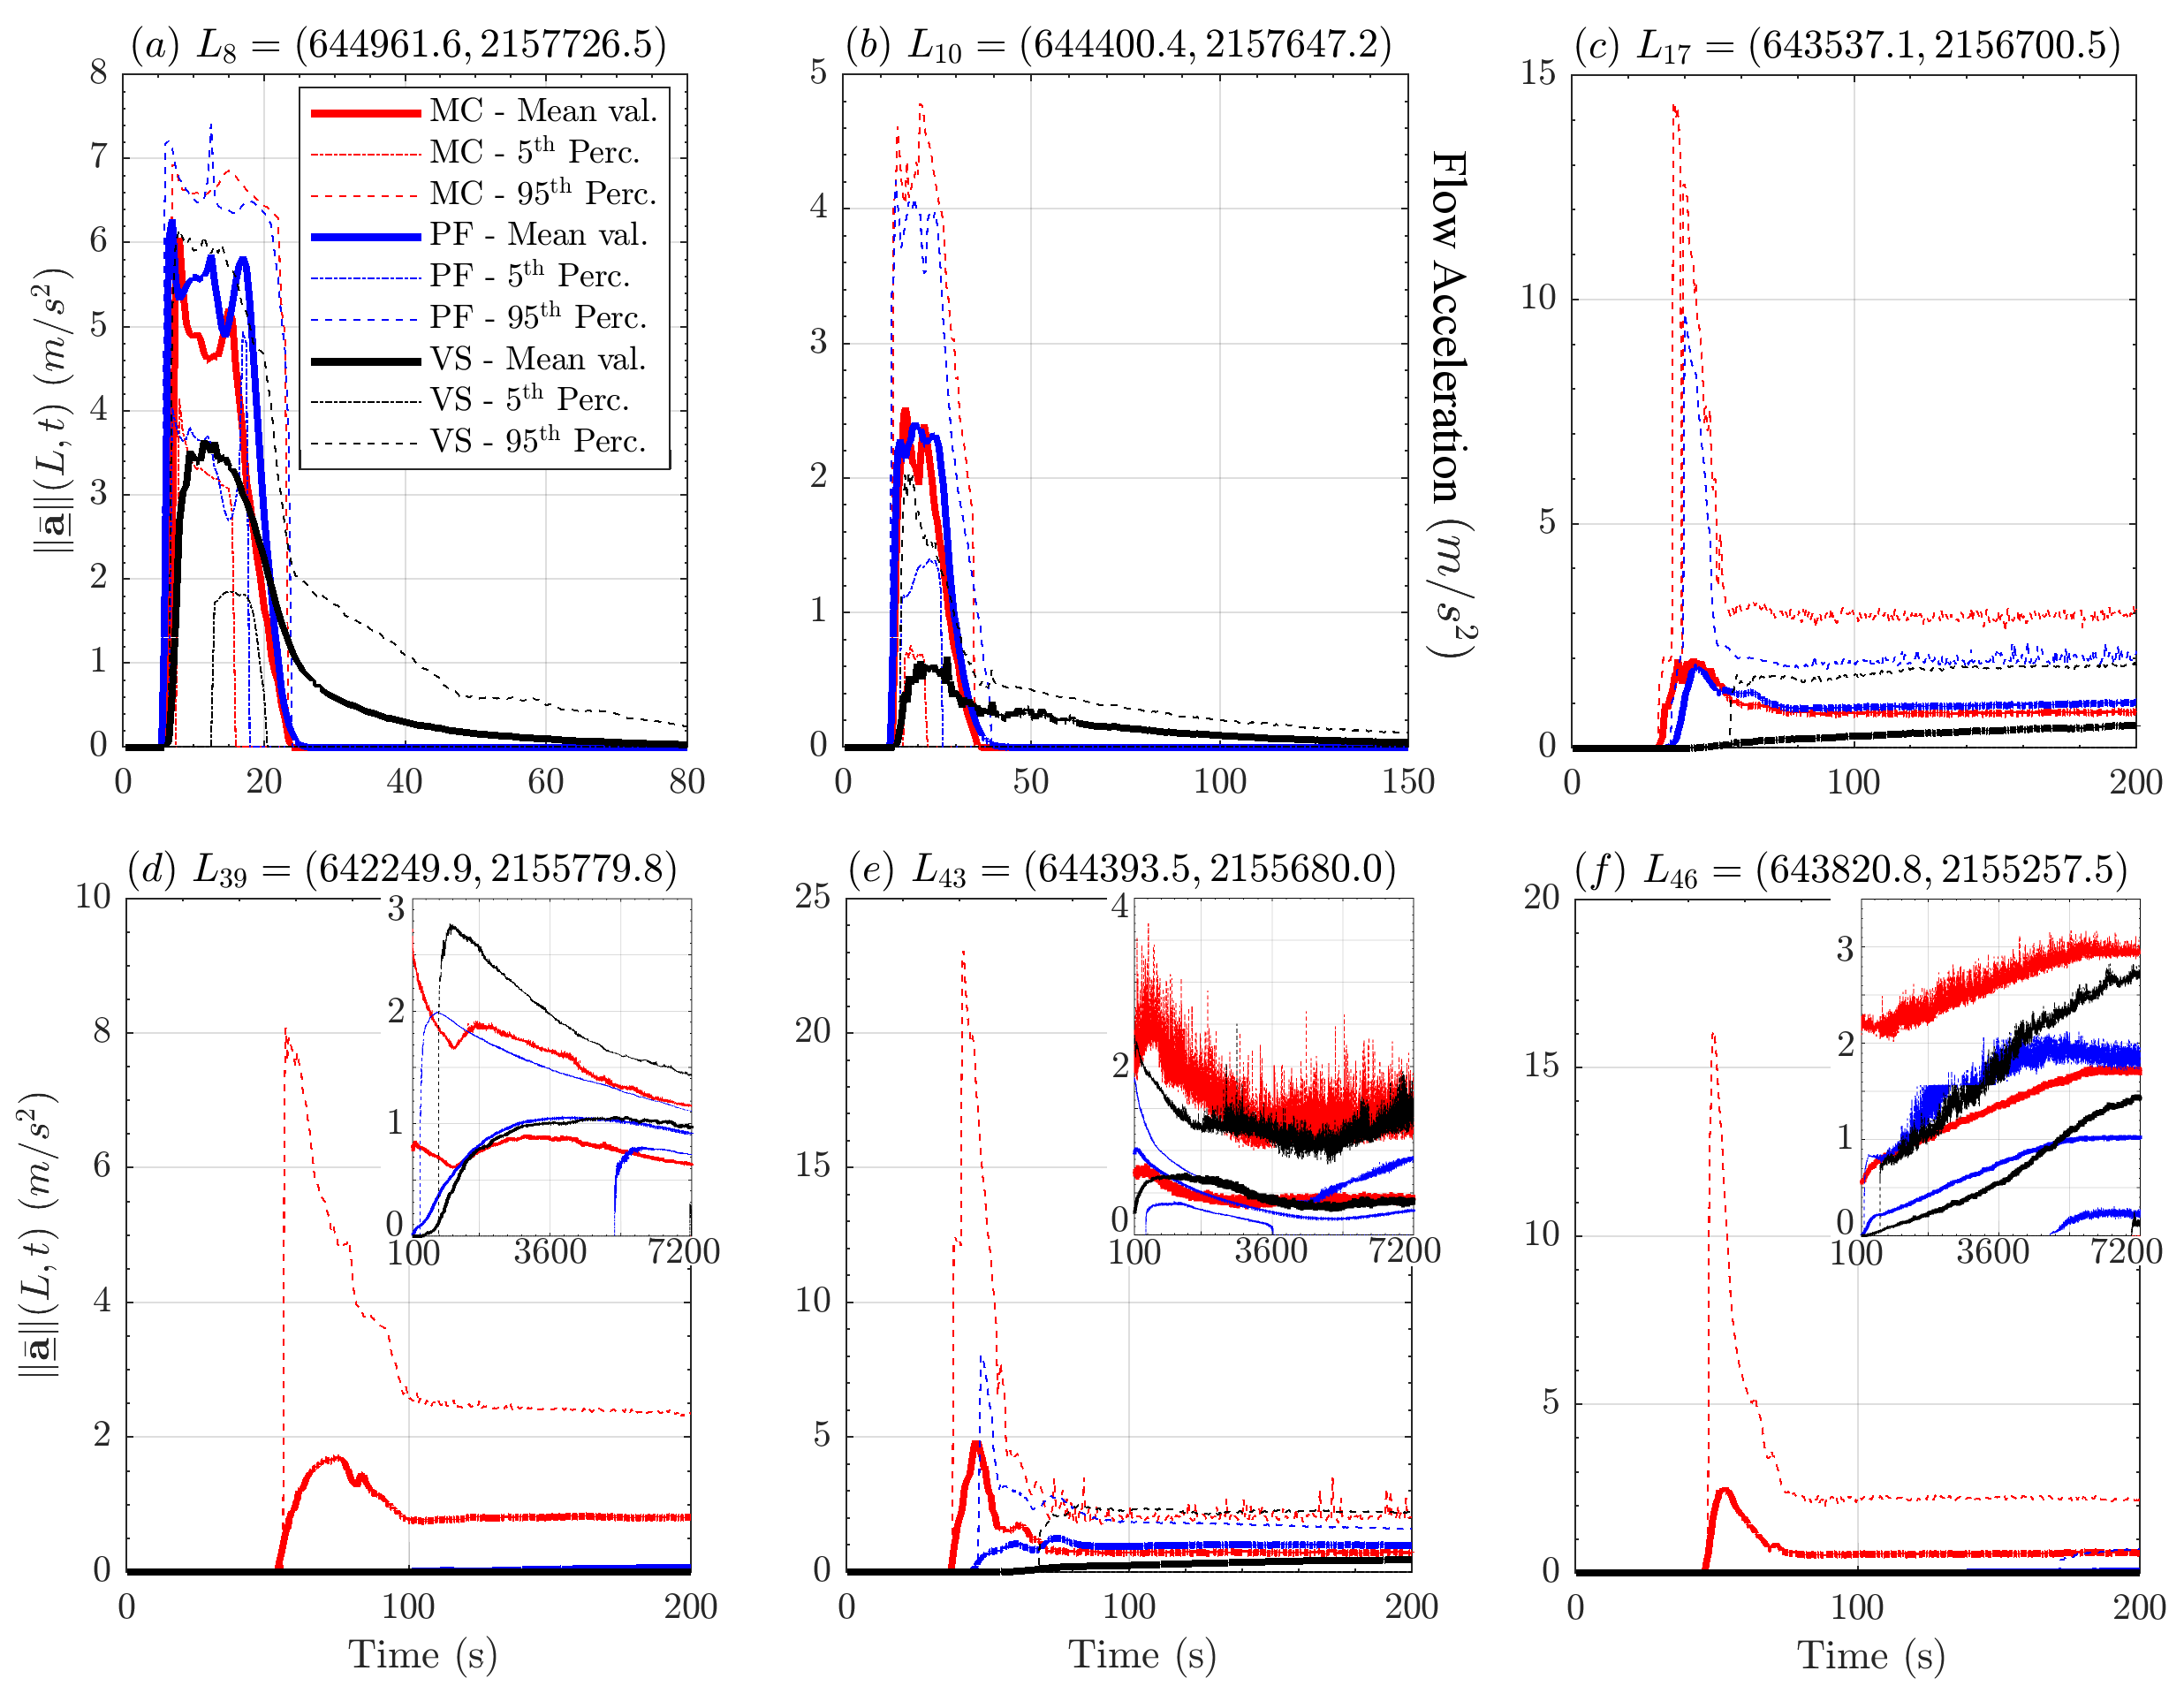
\includegraphics[width=1\textwidth]{BAF_VolcanDeColima/LocalMeasurments/Acceleration12.png}
        \caption{Records of flow acceleration magnitude (computed from LHS), in six selected locations. Records of points $L_{39}$, $L_{43}$, and $L_{46}$ are displayed at two different scales, according to the initial dynamics, in plots (d-f), and the asymptotic dynamics, in plots (g-i). Bold line is mean value, dashed lines are 5$^{\mathrm{th}}$ and 95$^{\mathrm{th}}$ percentile bounds. Different rheology models are displayed with different colors. Numerical noise affecting percentile curves in the small box of (f) has been averaged.}
        \label{fig:Colima-Accel1}
\end{figure}
In plot \ref{fig:Colima-Accel1}a,b, MC and PF display a higher maximum acceleration, both at $\sim 6 m/s^2$ and $\sim 2.5 m/s^2$ in the first and second plot respectively, than VS, $\sim 3.5 m/s^2$ and $\sim 0.5 m/s^2$, respectively. The latter has a slower decrease to zero. Uncertainty in VS is more significant in plot \ref{fig:Colima-Accel1}a, than in plot \ref{fig:Colima-Accel1}b. It is the opposite in MC and PF. In plot \ref{fig:Colima-Accel1}c, in MC and PF there can be a significant peak in acceleration, up to $\sim 15 m/s^2$ and $\sim 10 m/s^2$, in the 95$^{th}$ percentile values, respectively. The same peak is absent in the average plots, which are significantly flat in all the models, displaying values at $\sim 1 m/s^2$ in MC and PF, and $\sim 0.5 m/s^2$ in VS, at $\sim 200 s$. Plot \ref{fig:Colima-Accel1}e is similar, but PF is significantly reduced and lacks of the peak in the 95$^{th}$ percentile values. In plot \ref{fig:Colima-Accel1}d,f, only MC shows significant acceleration values. Plots \ref{fig:Colima-Accel1}g,h,i, are a zoom on the acceleration values in the distal locations, displayed on a long time window of $7200 s$. The last two plots are more noisy, but possess an increasing trend. All the three show, in all the models, values up to $\sim 1 m/s^2$. In general, PF acceleration tends to be lower than in the other models.

\subsection{Force contribution coefficients}
Figure \ref{fig:Colima-Ci_1} shows the Contributions Coefficients $(C_i)_{i=1,\dots,4}$, for the three rheology models and focusing on the RHS terms modulus. The different models are plotted separately: \ref{fig:Colima-Ci_1}a,d,g assume MC; \ref{fig:Colima-Ci_1}b,e,h assume PF; \ref{fig:Colima-Ci_1}c,f,i assume VS.
\begin{figure}[H]
         \centering
        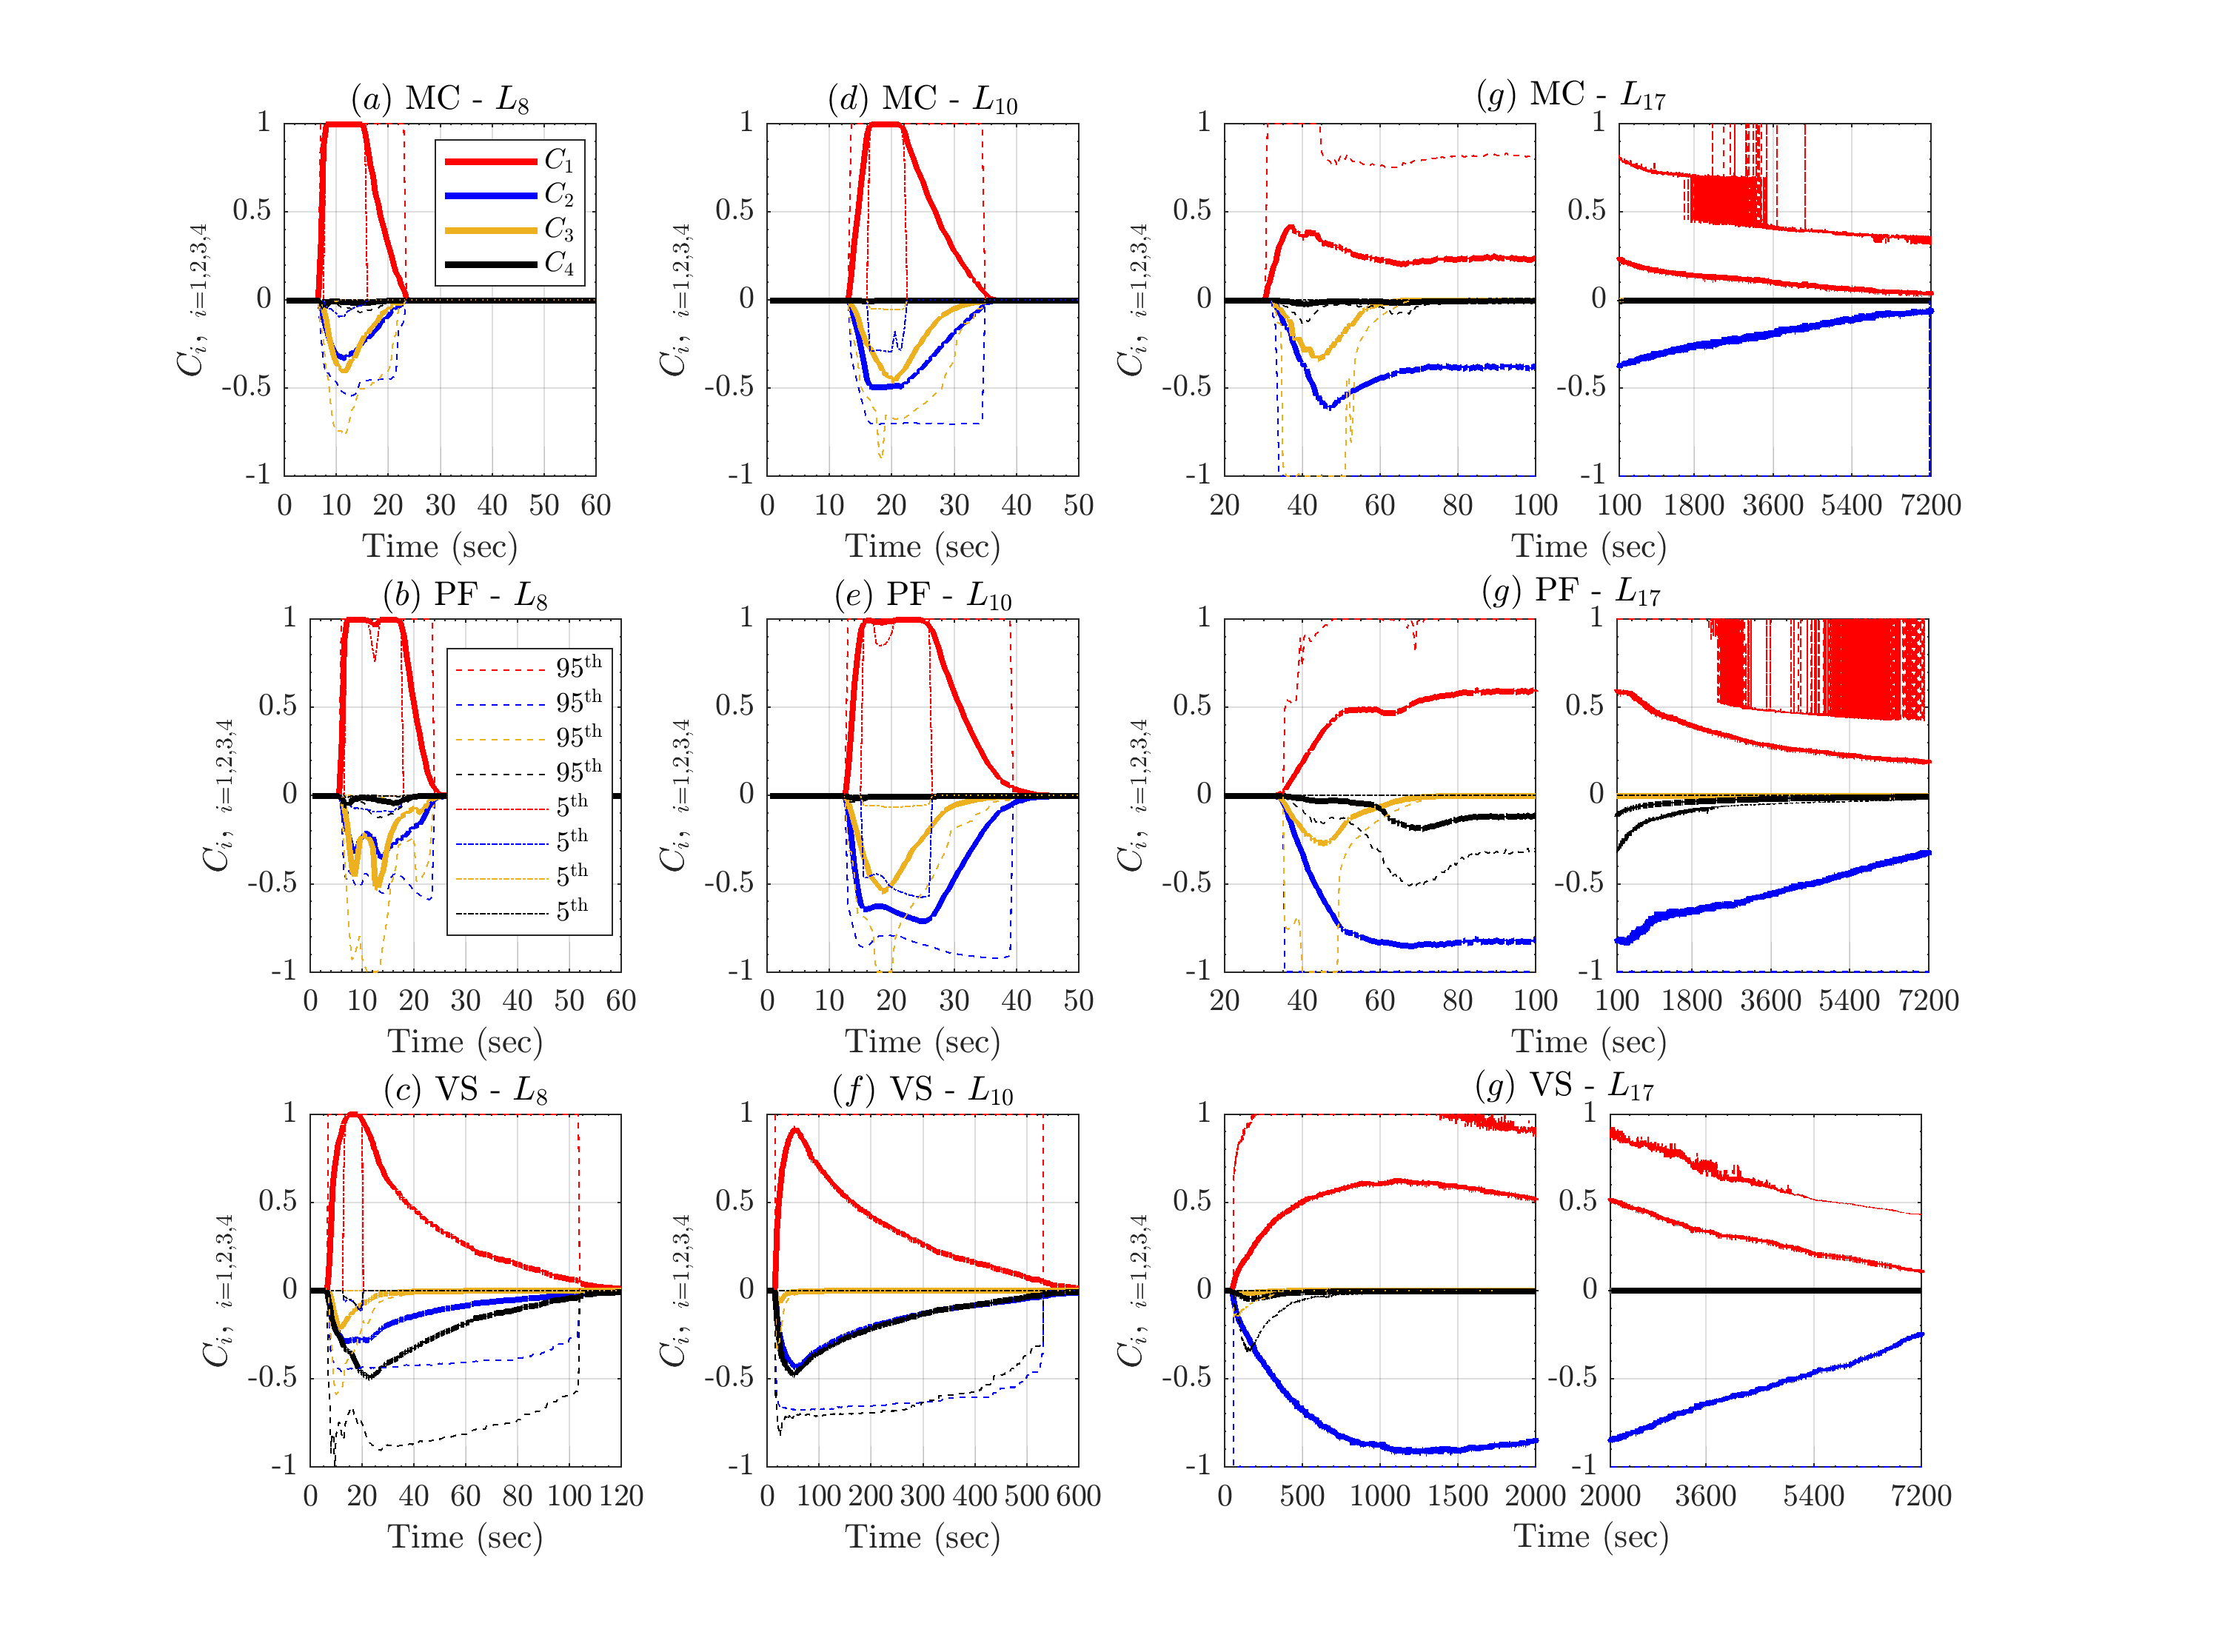
\includegraphics[width=1\textwidth]{BAF_VolcanDeColima/ForceContrib/Ci1_total.png}
        \caption{Records of contribution coefficients of \textbf{RHS} force moduli, at three spatial locations of interest, in the first km of runout. Different rheology models are displayed with different colors. Dominant factor is calculated based on the $l^\infty$ norm}
        \label{fig:Colima-Ci_1}
\end{figure}
The coefficients in the first two locations, points $L_8$ and $L_{10}$, are shown in \ref{fig:Colima-Ci_1}a,b,c and \ref{fig:Colima-Ci_1}d,e,f, respectively. Those points are close to the initial pile, in the western and eastern sectors of the inundated area. The pairs of plots related to the same model are similar. In all the models the greater contribution is given by $C_1$, significantly larger than $C_2$ and $C_3$, which have similar scales in MC and PF, while $C_2>C_3$ in VS. $C_4$ always gives a negligible contribution, except for in VS, where it is comparable with $C_2$. In $L_8$, following PF, $C_3$ is bimodal, whereas the plot is unimodal in MC and VS, or in $L_{10}$. In $L_8$, $C_3$ is greater than in $L_{10}$, compared to the other forces. VS shows a slower decrease of the plots, which is due to the rising probability of no-flow. In plots \ref{fig:Colima-Ci_1}g,h,i, are shown the coefficients in $L_{17}$, about 1 km from the initial pile (in horizontal projection). The plots are split in two sub-frames, following different temporal scales - the first $100 s$ are on the left, and the rest of the temporal domain $[100, 7200] s$ is on the right. Initial dynamics is dominated by $C_2$, except for in MC, and only for a short time, $[30, 35] s$. In MC there is an initial peak of $C_2$ which is not observed in the other models.  $C_3$ has a significant size, in MC and PF, and unimodal profile. In PF, after $C_3$ wanes, at about $60 s$, also $C_4$, representing the effect of hydrostatic pressure correction, is not negligible, for $\sim 40 s$. The second part of the temporal domain, is characterized by a slow decrease of $C_2>C_1$, due to the rise of the no-flow probability.

The current case study does not show a preferential direction, equivalent to the slope direction of the inclined plane. Hence, we will focus on the moduli of the force terms.
\subsection{Force terms}
Figure \ref{fig:Colima-F-spatial} shows the spatial sum of the force terms moduli, for the three rheology models.
\begin{figure}[H]
        \centering
        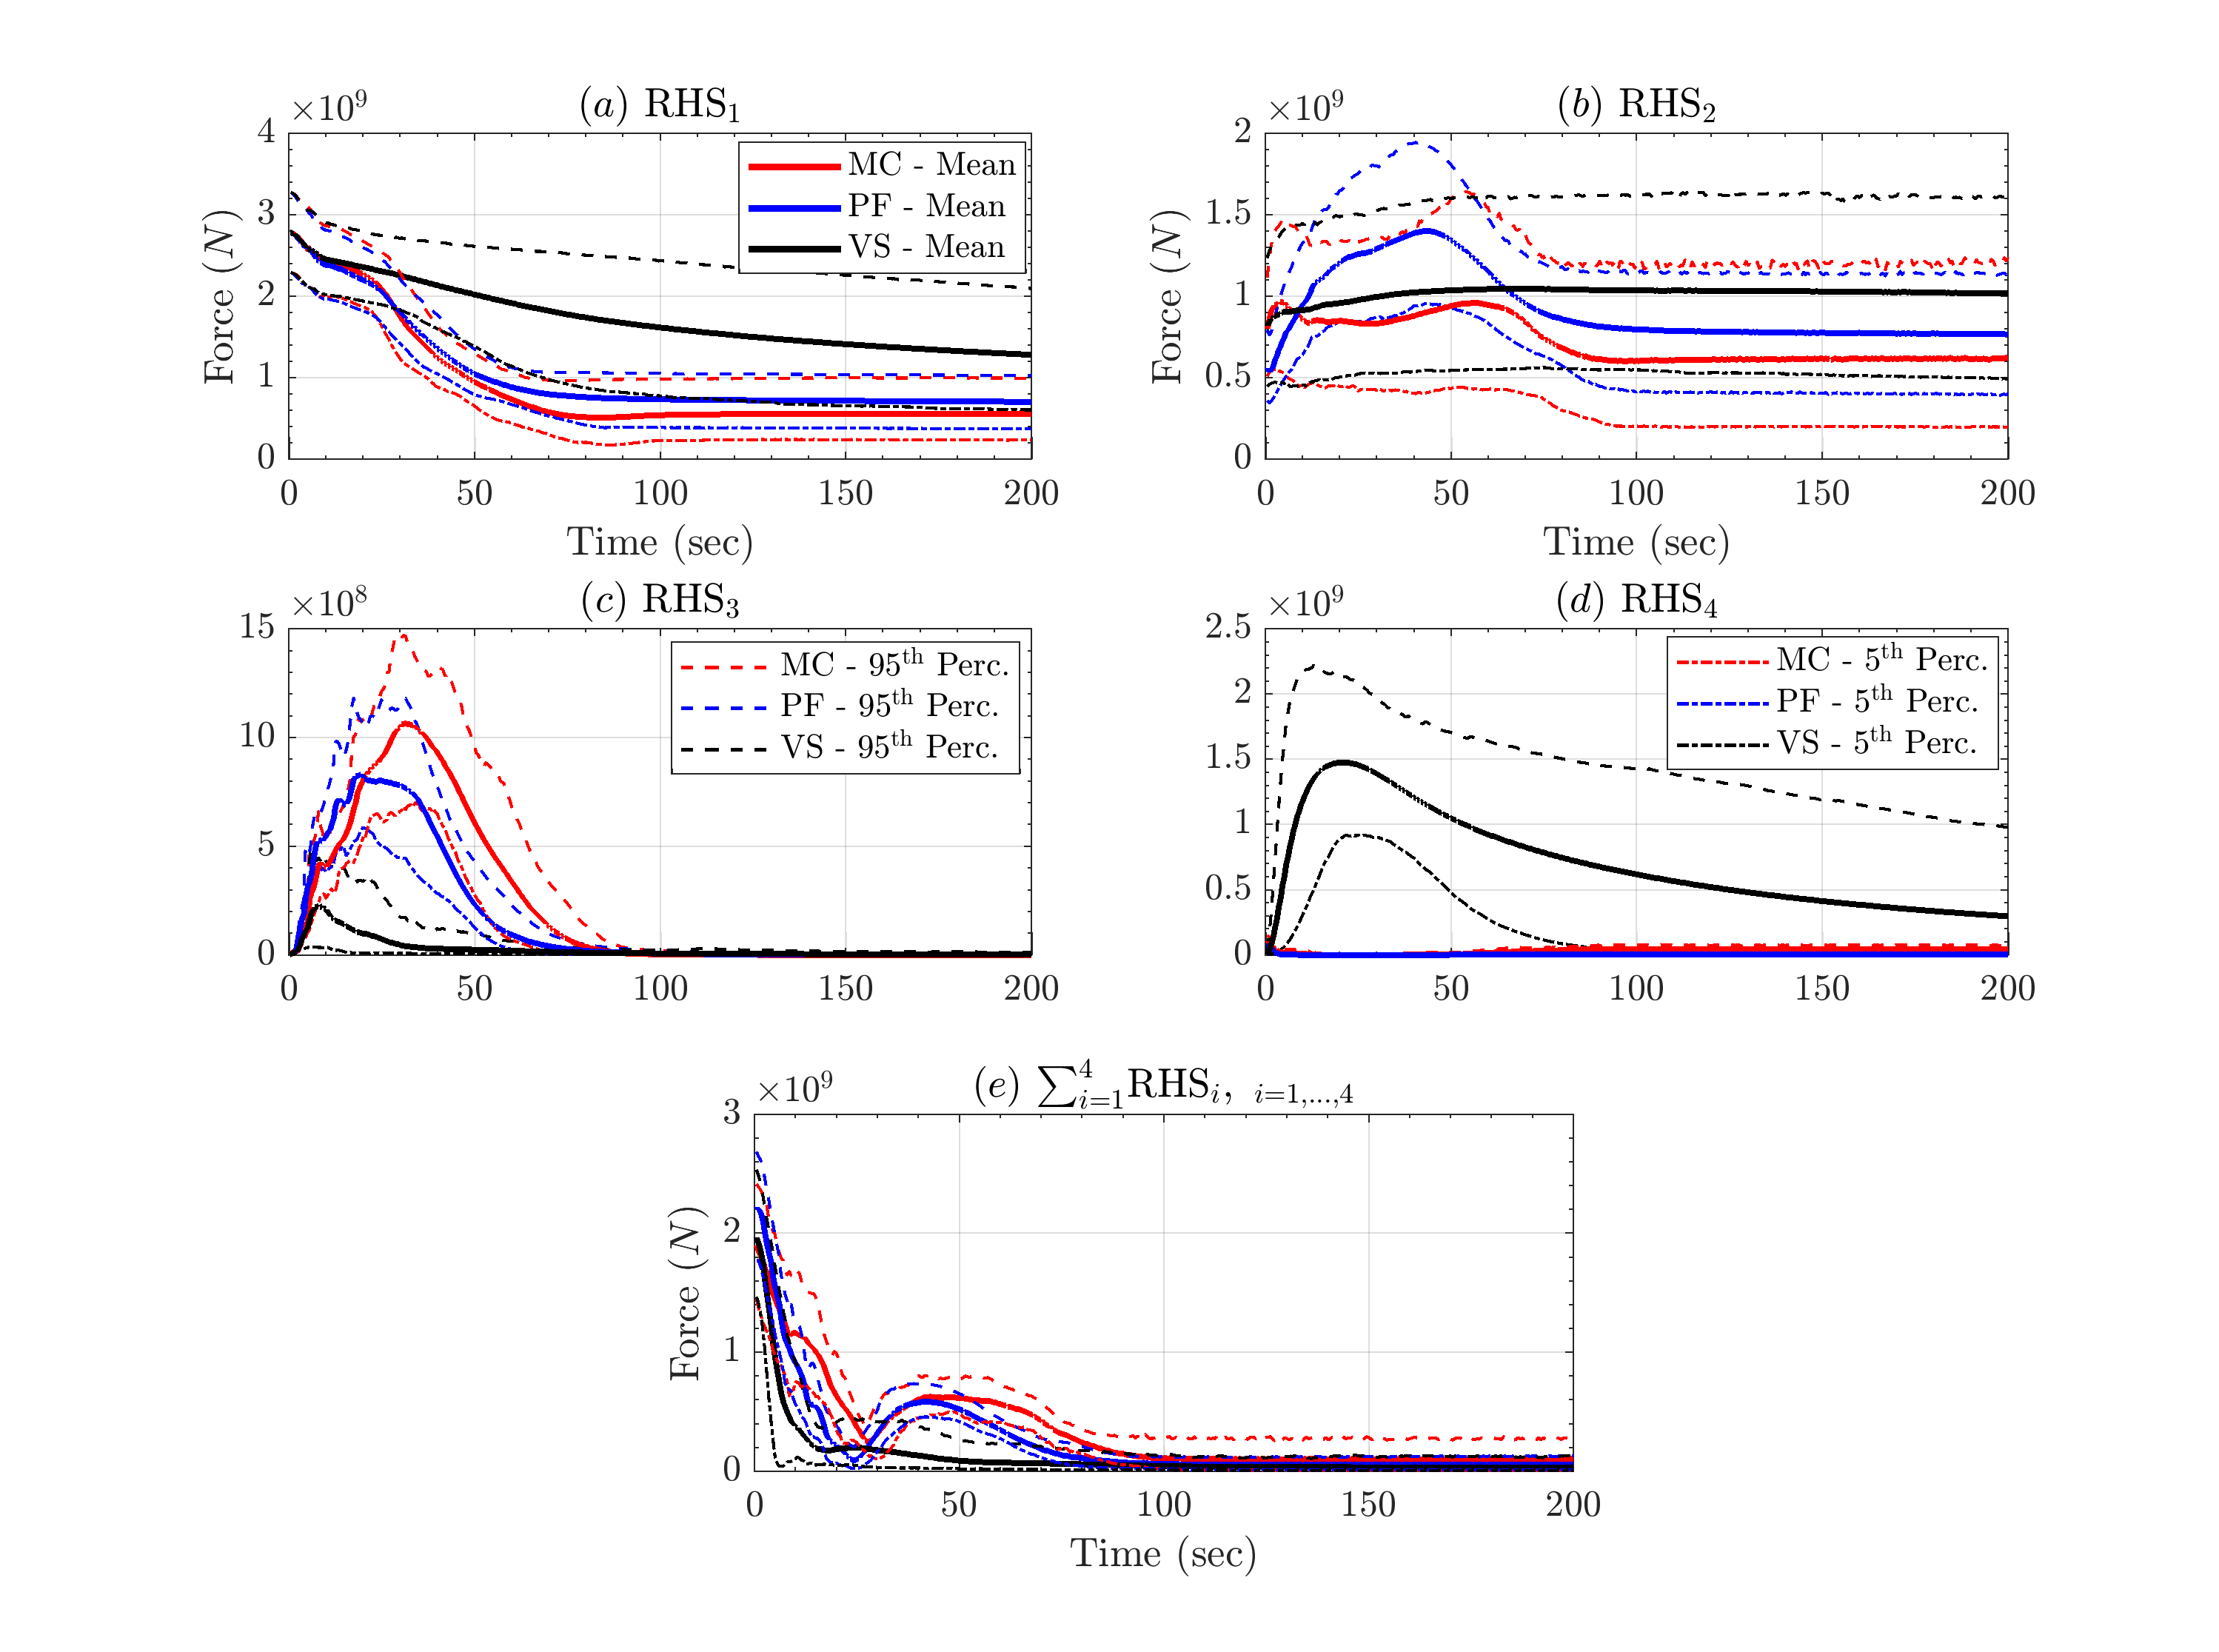
\includegraphics[width=1\textwidth]{BAF_VolcanDeColima/AveragedMeasurments/ForcesColima.png}
        \caption{Spatial sum of the RHS force terms moduli. Bold line is mean value, dashed lines are 5$^{\mathrm{th}}$ and 95$^{\mathrm{th}}$ percentile bounds.}
        \label{fig:Colima-F-spatial}
\end{figure}
The figure can be compared with Fig. \ref{fig:Ramp-Fx-spatial}, which was related to forces in the slope direction in the inclined plane case study. In plot \ref{fig:Colima-F-spatial}a $\boldsymbol{RHS_1}$ represents the effect of the gravity in all the models. It is decreasing in all the models, but more gradually in VS than in the others. Initial values are $2.8e9 N$ in all the models, uncertainty $\pm 2.5e8 N$. Force values are consistent with the material weight component along the mountain slope, and their decrease is related to the slope reduction. At $\sim 10 s$ all the models show a slowing down of the decrease, which is permanent in VS, and lasting $10 s$ in MC and PF. The latter models, reach a flat profile after $\sim 60 s$, at $6e8 N$ and $7e8 N$, respectively, and uncertainty of $\pm 2e8 N$ and $1.5e8 N$. VS, which flattens more gradually, is $1.3e9 N$ at $200 s$, uncertainty $[-7e8,+8e8] N$. In plot  \ref{fig:Colima-F-spatial}b $\boldsymbol{RHS_2}$ represents the effect of the basal friction in all the models. In MC, shows a bimodal profile, with a peak at $5 s$, and a second one at $60 s$. Both of them at $9.5e8 N$ on average, with uncertainty of $[-4e8,+5e8] N$ in the first peak, and $[-5e8,+7e8] N$ in the second. The minimum between the two peaks is at $8e8 N$ and lasts from $10 s$ to $30 s$. After the second peak there is significant decrease, reaching $6e8 N$ at $90 s$, and becoming flat. Final uncertainty is $[-4e8, +6e8] N$. In PF, the plot starts from lower initial values than in the other models, but then has a unimodal peak of $1.4e9 N$ at $40 s$, on average. Uncertainty $\pm 5e8 N$. After that, the plot decreases, reaching $7.5e8 N$ at $90 s$, and becoming flat. Final uncertainty is $\pm 3.5e8 N N$, lower than in the other models. In VS, there is slow increase until the plot reaches $1.05e9 N$ at $70 s$. Then the average force is almost flat, at $1.0e9 N$, with significant uncertainty of $[-5e8,+6e8] N$. In plot \ref{fig:Colima-F-spatial}c $\boldsymbol{RHS_3}$ represents the effect of the curvature of terrain. The three models all show a bell-shaped profile, waning to zero at $90 s$. However, MC reaches $1.1e9 N$ at $30 s$, PF $8e8 N$ at $20 s$, VS $2.5e8 N$ at $10 s$. The rise has a similar profile, but a different duration. The decrease is more gradual in VS. Uncertainty at the peak value is $\pm 4.5e8 N$ in MC, $[-2.5e8,+3.5e8] N$ in PF, $\pm 2e8 N$ in VS. In plot \ref{fig:Colima-F-spatial}d $\boldsymbol{RHS_4}$ has a different meaning in the three models. In MC it is the internal friction term, and it has a small peak in the first second, at $1e8 N$. After that it flattens to negligible values, but shows again values at $5e7 N$ after $60 s$. In PF it is the a depth averaged correction in the hydrostatic pressure, and has a almost negligible effect only in the first second, at $5e7 N$. In VS, instead, it is the velocity dependent term, and has a very relevant effect. The plot shows a bell-shaped profile, with a peak of $1.45e9 N$ at $20 s$. Uncertainty is $[-5.5e8, +6.6e8] N$, at the peak. After that, the force gradually decreases, and is $3e8 N$ at $200 s$, on average. Uncertainty $[-3e8, +7e8] N$. In plot \ref{fig:Colima-F-spatial}e, the modulus of the total force $\sum^4_{i=1}\boldsymbol{RHS_i}$ is shown, with the complex interplay between the terms. First a steep decrease due to the domination of the gravity upon the friction, then a bell-shaped increase when the friction stops the dynamics.
\end{document} 